\documentclass{article}
                  \usepackage{amsmath}
                 \usepackage[dvips]{graphicx}
                    \graphicspath{{./}{/home/art/univer_docs/sem5/automatization/dz/17/img}}
                  \DeclareGraphicsExtensions{.pdf, .png, .jpg}
                 \setlength{\tabcolsep}{4pt}                   \setlength{\columnsep}{4pt}                   \usepackage{mathtext}
                    \usepackage[english,russian]{babel}
                  \usepackage[T2A]{fontenc}
                    \usepackage[utf8]{inputenc}
                  \setcounter{MaxMatrixCols}{20}
                   \begin{document}
Условие задания:

\begin{figure}[h]
\center{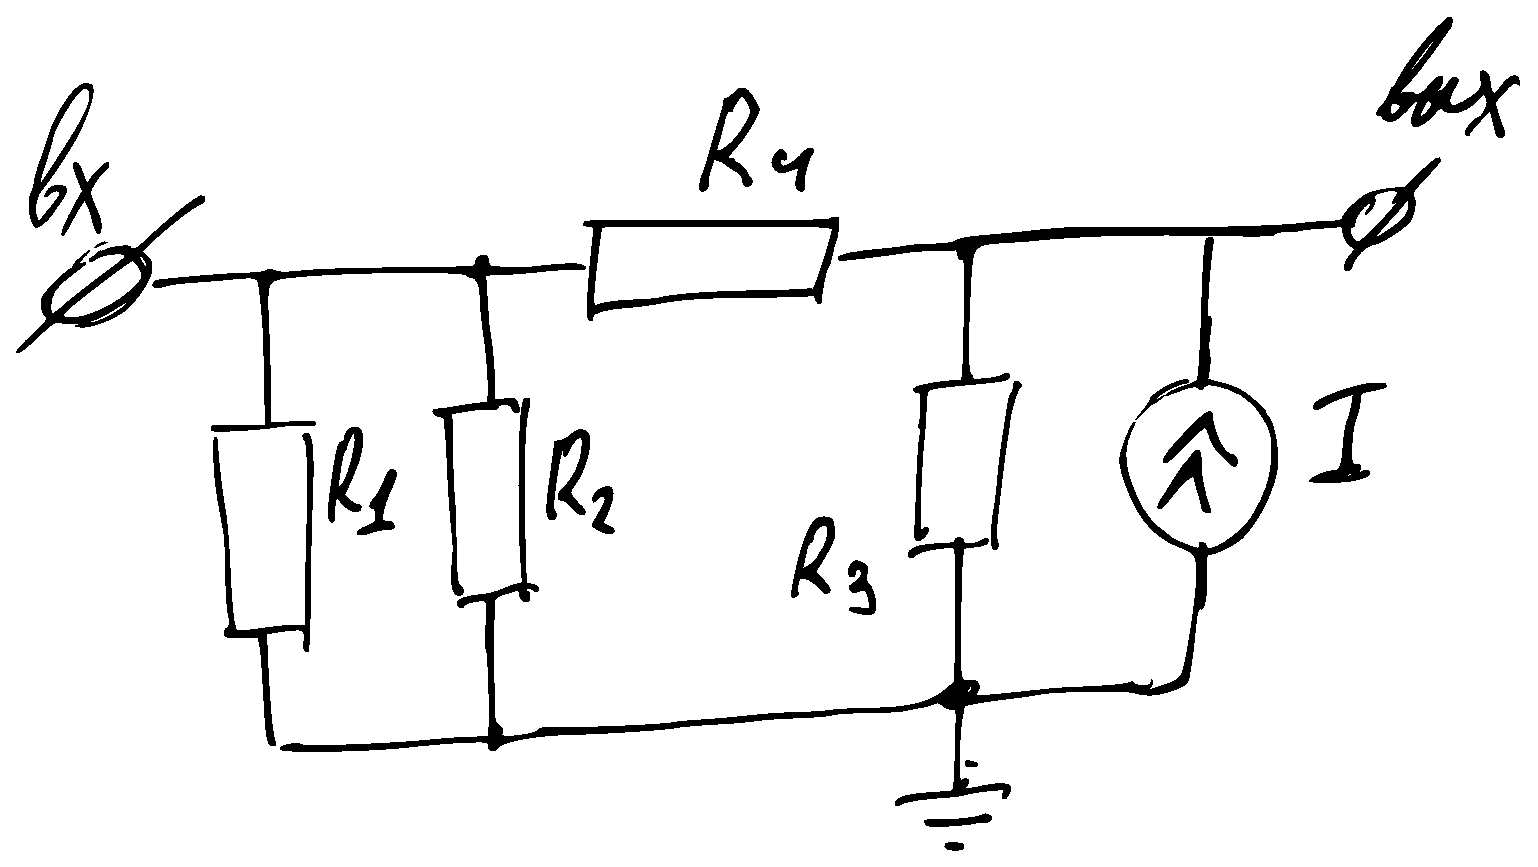
\includegraphics[height=0.25\textheight]{./../u.eps}}
\end{figure}
Коммутационная схема:

\begin{figure}[h]
\center{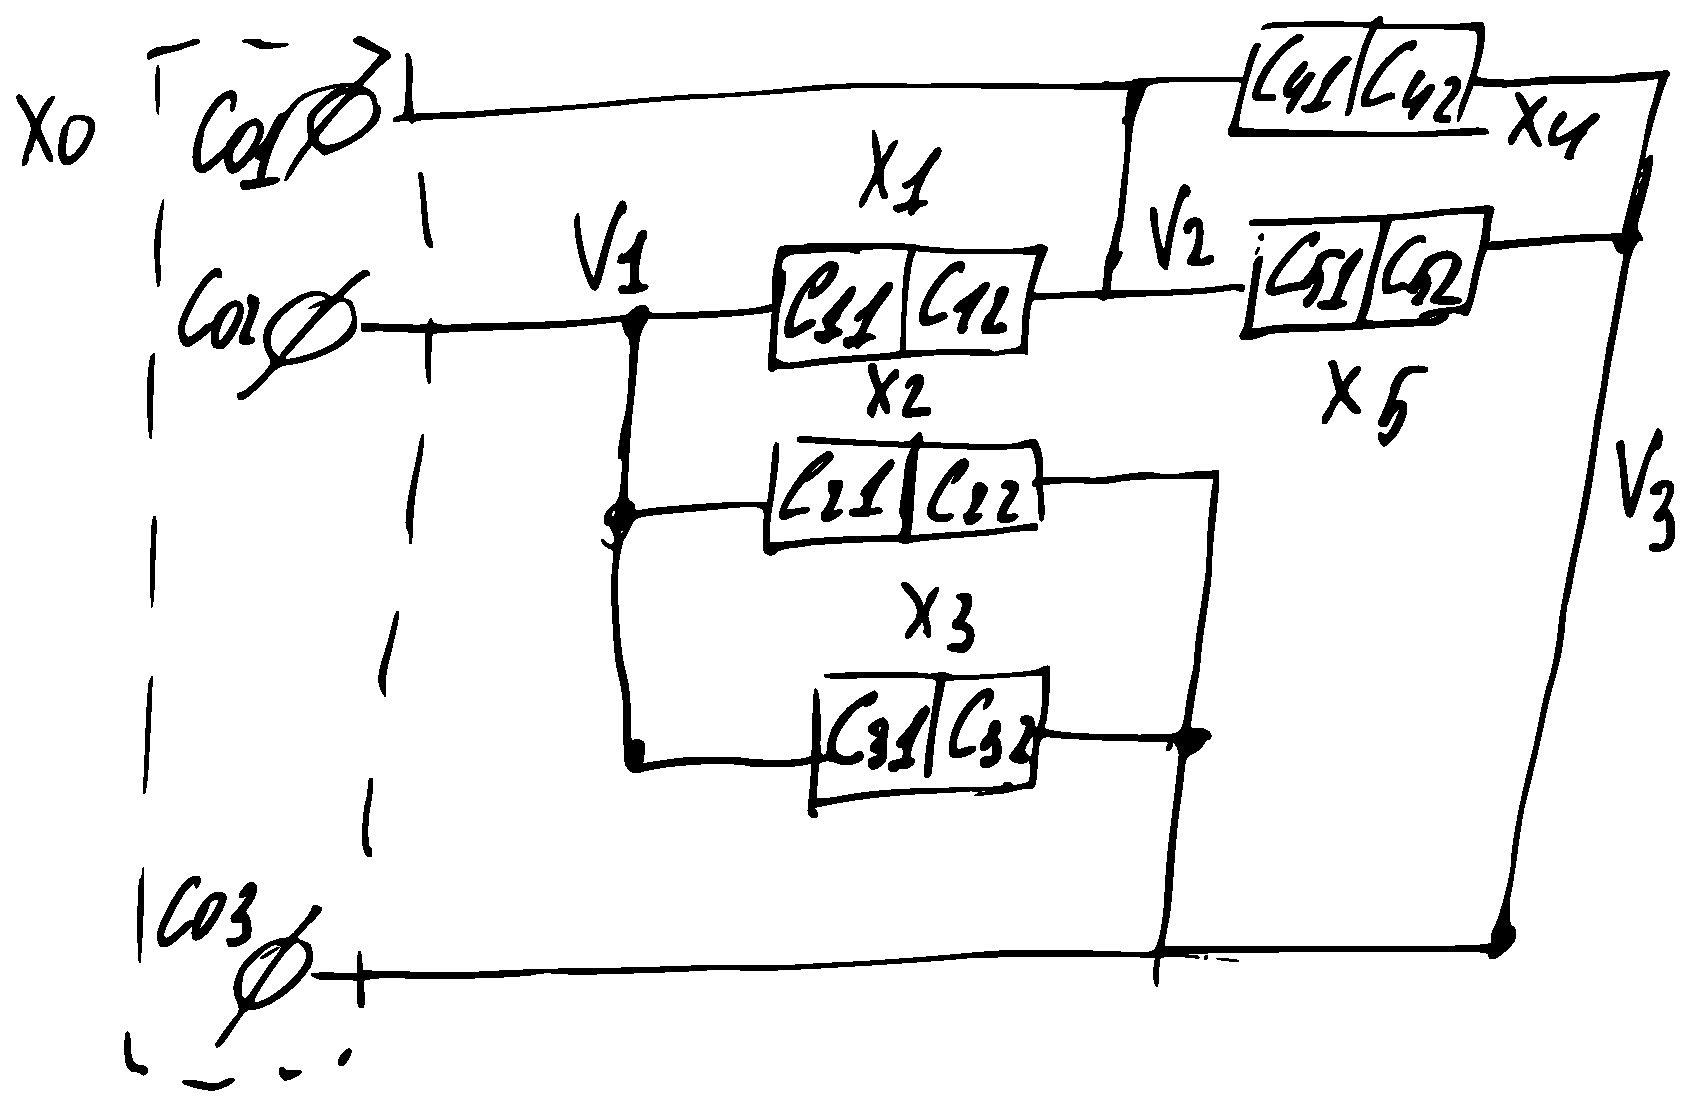
\includegraphics[height=0.25\textheight]{./../k.eps}}
\end{figure}
Список цепей:
\begin{tabular}{|c|c|c|}

\hline $V_{1}$ &$x_{1}$, $x_{2}$, $x_{0}$, $x_{3}$ & $C_{02}$, $C_{21}$, $C_{31}$, $C_{11}$ \cr\hline $V_{2}$ &$x_{1}$, $x_{0}$, $x_{4}$, $x_{5}$ & $C_{01}$, $C_{41}$, $C_{51}$, $C_{12}$ \cr\hline $V_{3}$ &$x_{4}$, $x_{0}$, $x_{3}$, $x_{2}$, $x_{5}$ & $C_{03}$, $C_{52}$, $C_{32}$, $C_{22}$, $C_{42}$ \cr\hline
\end{tabular}

Граф коммутационной схемы:

\begin{figure}[h]
\center{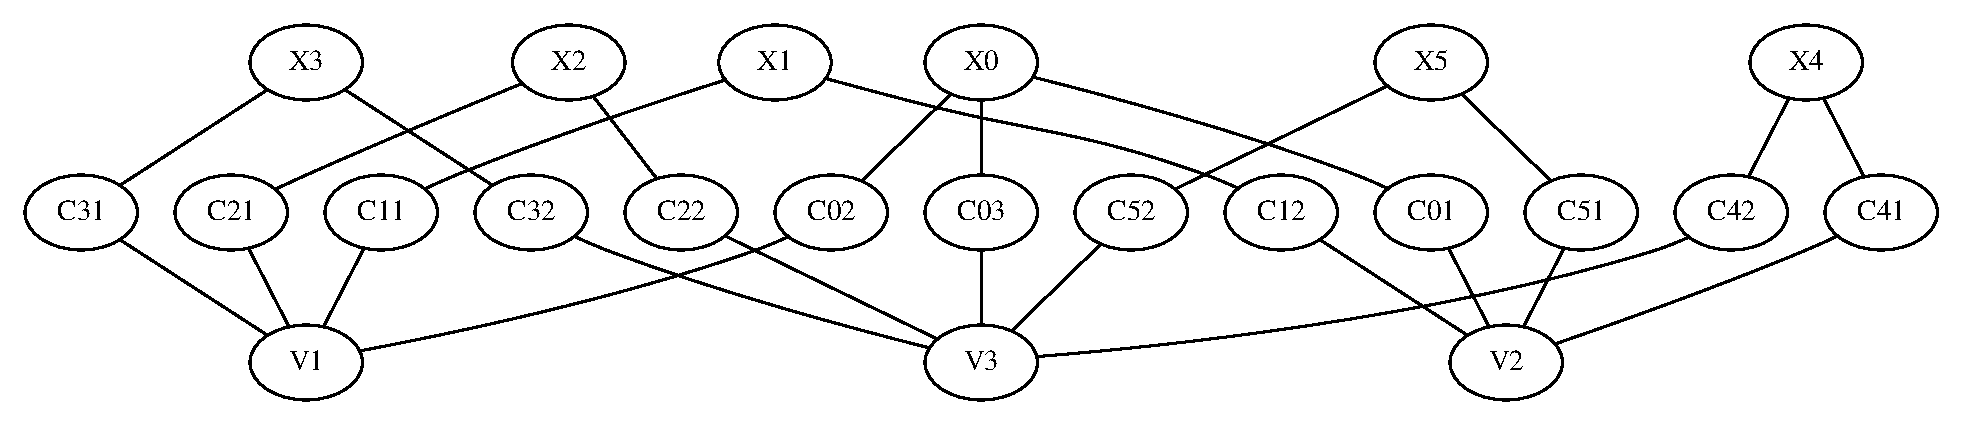
\includegraphics[width=\linewidth]{test.eps}}
\end{figure}
$$
 A =
\bordermatrix{ & C_{01} \!&\! C_{02} \!&\! C_{03} \!&\! C_{11} \!&\! C_{12} \!&\! C_{21} \!&\! C_{22} \!&\! C_{31} \!&\! C_{32} \!&\! C_{41} \!&\! C_{42} \!&\! C_{51} \!&\! C_{52} \!&\! \cr 
V_{1} \!&\! 0 \!&\! 1 \!&\! 0 \!&\! 1 \!&\! 0 \!&\! 1 \!&\! 0 \!&\! 1 \!&\! 0 \!&\! 0 \!&\! 0 \!&\! 0 \!&\! 0 \!&\! \cr
V_{2} \!&\! 1 \!&\! 0 \!&\! 0 \!&\! 0 \!&\! 1 \!&\! 0 \!&\! 0 \!&\! 0 \!&\! 0 \!&\! 1 \!&\! 0 \!&\! 1 \!&\! 0 \!&\! \cr
V_{3} \!&\! 0 \!&\! 0 \!&\! 1 \!&\! 0 \!&\! 0 \!&\! 0 \!&\! 1 \!&\! 0 \!&\! 1 \!&\! 0 \!&\! 1 \!&\! 0 \!&\! 1 \!&\! \cr
}$$
$$
B =
\bordermatrix{ & C_{01} \!&\! C_{02} \!&\! C_{03} \!&\! C_{11} \!&\! C_{12} \!&\! C_{21} \!&\! C_{22} \!&\! C_{31} \!&\! C_{32} \!&\! C_{41} \!&\! C_{42} \!&\! C_{51} \!&\! C_{52} \!&\! \cr 
x_{0} \!&\! 1 \!&\! 1 \!&\! 1 \!&\! 0 \!&\! 0 \!&\! 0 \!&\! 0 \!&\! 0 \!&\! 0 \!&\! 0 \!&\! 0 \!&\! 0 \!&\! 0 \!&\! \cr
x_{1} \!&\! 0 \!&\! 0 \!&\! 0 \!&\! 1 \!&\! 1 \!&\! 0 \!&\! 0 \!&\! 0 \!&\! 0 \!&\! 0 \!&\! 0 \!&\! 0 \!&\! 0 \!&\! \cr
x_{2} \!&\! 0 \!&\! 0 \!&\! 0 \!&\! 0 \!&\! 0 \!&\! 1 \!&\! 1 \!&\! 0 \!&\! 0 \!&\! 0 \!&\! 0 \!&\! 0 \!&\! 0 \!&\! \cr
x_{3} \!&\! 0 \!&\! 0 \!&\! 0 \!&\! 0 \!&\! 0 \!&\! 0 \!&\! 0 \!&\! 1 \!&\! 1 \!&\! 0 \!&\! 0 \!&\! 0 \!&\! 0 \!&\! \cr
x_{4} \!&\! 0 \!&\! 0 \!&\! 0 \!&\! 0 \!&\! 0 \!&\! 0 \!&\! 0 \!&\! 0 \!&\! 0 \!&\! 1 \!&\! 1 \!&\! 0 \!&\! 0 \!&\! \cr
x_{5} \!&\! 0 \!&\! 0 \!&\! 0 \!&\! 0 \!&\! 0 \!&\! 0 \!&\! 0 \!&\! 0 \!&\! 0 \!&\! 0 \!&\! 0 \!&\! 1 \!&\! 1 \!&\! \cr
}$$
Граф элементных комплексов:
\begin{figure}[h]
\center{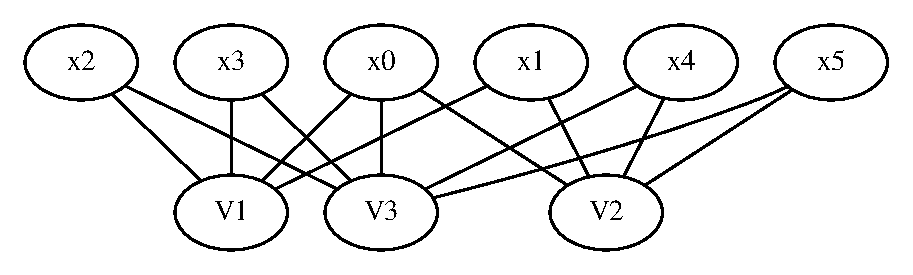
\includegraphics[width=\linewidth]{q.eps}}
\end{figure}
$$
Q =
\bordermatrix{ & V_{1} \!&\! V_{2} \!&\! V_{3} \!&\! \cr 
x_{0} \!&\! 1 \!&\! 1 \!&\! 1 \!&\! \cr
x_{1} \!&\! 1 \!&\! 1 \!&\! 0 \!&\! \cr
x_{2} \!&\! 1 \!&\! 0 \!&\! 1 \!&\! \cr
x_{3} \!&\! 1 \!&\! 0 \!&\! 1 \!&\! \cr
x_{4} \!&\! 0 \!&\! 1 \!&\! 1 \!&\! \cr
x_{5} \!&\! 0 \!&\! 1 \!&\! 1 \!&\! \cr
}$$
Взвешенный граф схемы:
\begin{figure}[h!]
\center{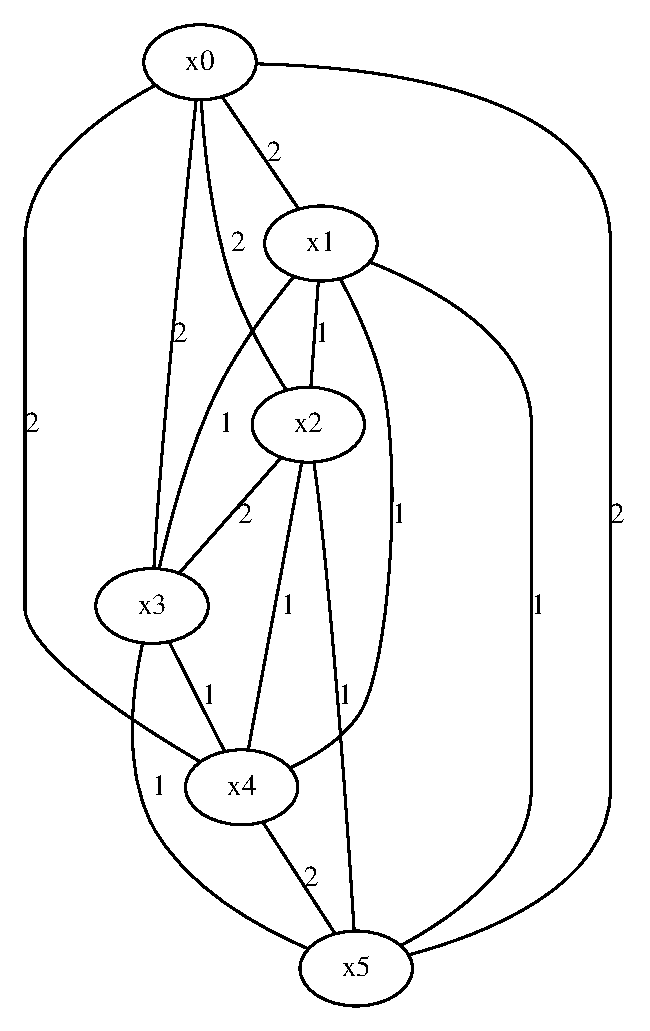
\includegraphics[height=0.25\textheight]{r.eps}}
\end{figure}
$$
R =
\bordermatrix{ & x_{0} \!&\! x_{1} \!&\! x_{2} \!&\! x_{3} \!&\! x_{4} \!&\! x_{5} \!&\! \cr 
x_{0} \!&\! 0 \!&\! 2 \!&\! 2 \!&\! 2 \!&\! 2 \!&\! 2 \!&\! \cr
x_{1} \!&\! 2 \!&\! 0 \!&\! 1 \!&\! 1 \!&\! 1 \!&\! 1 \!&\! \cr
x_{2} \!&\! 2 \!&\! 1 \!&\! 0 \!&\! 2 \!&\! 1 \!&\! 1 \!&\! \cr
x_{3} \!&\! 2 \!&\! 1 \!&\! 2 \!&\! 0 \!&\! 1 \!&\! 1 \!&\! \cr
x_{4} \!&\! 2 \!&\! 1 \!&\! 1 \!&\! 1 \!&\! 0 \!&\! 2 \!&\! \cr
x_{5} \!&\! 2 \!&\! 1 \!&\! 1 \!&\! 1 \!&\! 2 \!&\! 0 \!&\! \cr
}$$
Расширенная таблица соединений:

$$
 Z =\left(
\begin{array}{cccccccccccccccccccccccccccccc}
1 \!&\! 2 \!&\! 3 \!&\! 4 \!&\! 5 \!&\! 0 \!&\! 2 \!&\! 3 \!&\! 4 \!&\! 5 \!&\! 0 \!&\! 1 \!&\! 3 \!&\! 4 \!&\! 5 \!&\! 0 \!&\! 1 \!&\! 2 \!&\! 4 \!&\! 5 \!&\! 0 \!&\! 1 \!&\! 2 \!&\! 3 \!&\! 5 \!&\! 0 \!&\! 1 \!&\! 2 \!&\! 3 \!&\! 4 
\end{array}
\right)$$
$$
 W =\left(
\begin{array}{cccccccccccccccccccccccccccccc}
2 \!&\! 2 \!&\! 2 \!&\! 2 \!&\! 2 \!&\! 2 \!&\! 1 \!&\! 1 \!&\! 1 \!&\! 1 \!&\! 2 \!&\! 1 \!&\! 2 \!&\! 1 \!&\! 1 \!&\! 2 \!&\! 1 \!&\! 2 \!&\! 1 \!&\! 1 \!&\! 2 \!&\! 1 \!&\! 1 \!&\! 1 \!&\! 2 \!&\! 2 \!&\! 1 \!&\! 1 \!&\! 1 \!&\! 2 
\end{array}
\right)$$
$$
 Z =\left(
\begin{array}{cccccc}
5 \!&\! 10 \!&\! 15 \!&\! 20 \!&\! 25 \!&\! 30 
\end{array}
\right)$$
\end{document}
